% Slide bảo vệ khóa luận tốt nghiệp — HSGE (Phiên bản in nộp: Không che mờ, không phụ lục).
% Build: latexmk -pdf main_print.tex
\documentclass[aspectratio=169,handout]{beamer}
% Preamble: document class, theme, Vietnamese support, shared macros.
\documentclass[aspectratio=169]{beamer}

\usetheme{Antibes}
\usecolortheme{whale}

% Vietnamese: T5 encoding (vntex) + Latin Modern covers the beamer sans family.
\usepackage[utf8]{inputenc}
\usepackage[T5]{fontenc}
\usepackage{lmodern}
\usepackage{textcomp}

\usepackage{graphicx}
\usepackage{booktabs}
\usepackage{array}
\usepackage{xcolor}
\graphicspath{{images/}}

% No navigation symbols. Antibes stacks a section bar and a subsection bar in
% the headline; this deck has no subsections, so keep only the section bar and
% give the reclaimed vertical space back to the content.
\setbeamertemplate{navigation symbols}{}
\setbeamertemplate{headline}{%
  \begin{beamercolorbox}[ht=2.6ex,dp=1.2ex]{section in head/foot}
    \insertnavigation{\paperwidth}
  \end{beamercolorbox}
}
\setbeamertemplate{caption}[numbered]
\setbeamercolor{block title}{bg=structure.fg!15,fg=black}
\setbeamercolor{block body}{bg=structure.fg!5}

% Fixed-width column types reused by the result tables.
\newcolumntype{L}[1]{>{\raggedright\arraybackslash}p{#1}}
\newcolumntype{R}[1]{>{\raggedleft\arraybackslash}p{#1}}

% Caption line under a figure on a slide.
\newcommand{\figcap}[1]{\vspace{0.1cm}{\scriptsize\itshape #1}}

% Highlight for the key number of a slide.
\newcommand{\kw}[1]{\textbf{\color{structure.fg}#1}}

\title[HSGE]{Xây dựng dữ liệu và tinh chỉnh mô hình ngôn ngữ nhỏ\\cho tác nhân trí tuệ nhân tạo trên web}
\subtitle{HSGE - Hierarchical Skill-Graph Exploration}

\author[Bảo Kiệt - Tiến Phát]{
  \texorpdfstring{Trương Bảo Kiệt - 22127223 \\ Hồ Tiến Phát - 22127321}{Trương Bảo Kiệt, Hồ Tiến Phát}
}

\institute[HCMUS]{
  Giảng viên hướng dẫn: PGS.TS. Nguyễn Văn Vũ \\[0.2cm]
  \small Bộ môn Công nghệ Phần mềm \\
  Khoa Công nghệ Thông tin - Trường Đại học Khoa học Tự nhiên, ĐHQG-HCM
}

\date{Khóa luận tốt nghiệp - 2026}



\begin{document}

\begin{frame}[plain]
  \titlepage
\end{frame}

% Outline frame: chỉ hiển thị 6 đề mục chính, ẩn toàn bộ mục con
\begin{frame}{Nội dung báo cáo}
  \small
  \begin{columns}[t]
    \begin{column}{0.48\textwidth}
      \tableofcontents[sections={1-3},hideallsubsections]
    \end{column}
    \hfill
    \begin{column}{0.48\textwidth}
      \tableofcontents[sections={4-6},hideallsubsections]
    \end{column}
  \end{columns}
\end{frame}

% Show outline before each section
\AtBeginSection[]
{
  \begin{frame}{Nội dung báo cáo}
    \footnotesize
    \begin{columns}[t]
      \begin{column}{0.48\textwidth}
        \tableofcontents[sections={1-3},currentsection,hideothersubsections]
      \end{column}
      \hfill
      \begin{column}{0.48\textwidth}
        \tableofcontents[sections={4-6},currentsection,hideothersubsections]
      \end{column}
    \end{columns}
  \end{frame}
}

% !TEX root = ../main.tex

%%% ============================================================
\section{Giới thiệu}
%%% ============================================================

\subsection{Bối cảnh: khoảng cách hiệu năng trên tác vụ web}
\begin{frame}{Bối cảnh: khoảng cách hiệu năng trên tác vụ web}
  \framesubtitle{Mô hình càng lớn càng tốt --- nhưng tốt tới đâu, và trả giá bằng gì?}
  \begin{columns}[t]
    \begin{column}{0.52\textwidth}
      \uncover<1->{
        \head{Web agent: kỳ vọng và thực tế}
        \begin{itemize}\ilist
          \item \textbf{LLM phát triển} $\rightarrow$ thúc đẩy \textbf{web agent} tự động hóa thao tác trên trình duyệt.
          \item Trên \textbf{WebArena} (benchmark website thực): agent dùng \textbf{GPT-4} chỉ đạt \kw{14,41\%}, trong khi con người đạt \kw{78,24\%}.
          \item $\Rightarrow$ Năng lực tổng quát của LLM \kw{chưa đủ}; cần \kw{chuyên biệt hóa} theo môi trường triển khai.
        \end{itemize}
      }
    \end{column}

    \hfill
    \begin{column}{0.44\textwidth}
      \uncover<2->{
        \begin{block}{Vì sao không chỉ gọi LLM lớn qua API?}
          \begin{itemize}\isub
            \item \textbf{Chi phí} cao, \textbf{độ trễ} lớn khi chạy hàng loạt.
            \item \textbf{Rủi ro riêng tư}: dữ liệu nội bộ rời khỏi tổ chức.
          \end{itemize}
        \end{block}
      }

      \gap
      \uncover<3->{
        \begin{block}{Hướng đi: SLM ${<}10$B chạy cục bộ}
          \begin{itemize}\isub
            \item Rẻ, chủ động, dữ liệu không ra ngoài; nhưng năng lực gốc yếu $\rightarrow$ \kw{bắt buộc fine-tune}.
            \item $\Rightarrow$ Nút thắt chuyển từ \textbf{mô hình} sang \kw{dữ liệu huấn luyện}.
          \end{itemize}
        \end{block}
      }
    \end{column}
  \end{columns}
\end{frame}

\subsection{Thách thức dữ liệu \& các nghiên cứu liên quan}
\begin{frame}{Thách thức thu thập dữ liệu và các nghiên cứu trước}
  \framesubtitle{Lấy đâu ra trajectory để huấn luyện, khi không có người gán nhãn?}
  \begin{columns}[t]
    \begin{column}{0.40\textwidth}
      \uncover<1->{
        \head{Thách thức: chi phí dữ liệu}
        \begin{itemize}\ilist
          \item Gán nhãn tay: \textbf{AutoWebGLM} cần \kw{20 người $\times$ 1 tháng} cho ${\sim}10.000$ trajectory.
          \item Mẫu tổng hợp rẻ hơn: \textbf{Synatra} chỉ tốn \kw{${\sim}3\%$} chi phí mỗi mẫu.
          \item Nhưng dữ liệu \textbf{ngoại tuyến} không bám môi trường thật: \kw{6\%} (Synatra) so với \kw{16\%} (NNetNav) trên WebArena.
        \end{itemize}
      }
    \end{column}

    \hfill
    \begin{column}{0.57\textwidth}
      \uncover<2->{\head{Ba hướng nghiên cứu trước đây}}

      \gap
      \uncover<2->{
        \begin{block}{(A) Tri thức gián tiếp $\rightarrow$ trajectory}
          \scriptsize \textbf{Synatra}, \textbf{AgentTrek}: chuyển bài hướng dẫn / tài liệu trên Internet thành mẫu huấn luyện, replay trên trình duyệt thật.
        \end{block}
      }

      \uncover<3->{
        \begin{block}{(B) Bộ nhớ \& skill cho lúc suy luận}
          \scriptsize \textbf{AWM}: trích workflow lặp lại, nhét vào prompt --- WebArena \kw{23,5\% $\rightarrow$ 35,5\%}. \textbf{SkillWeaver}: agent tự khám phá, đóng gói skill thành API tái sử dụng.
        \end{block}
      }

      \uncover<4->{
        \begin{block}{(C) Tự khám phá $\rightarrow$ dữ liệu huấn luyện SLM}
          \scriptsize \textbf{NNetNav}: khám phá rồi gán nhãn hồi tố, 8B đạt \kw{16,3\%}. \textbf{Go-Browse}: khám phá như \textbf{tìm kiếm trên đồ thị} website, 7B đạt \kw{21,7\%} --- SOTA phân khúc ${<}10$B.
        \end{block}
      }
    \end{column}
  \end{columns}
\end{frame}

\subsection{Hạn chế của các phương pháp trước \& bài toán đặt ra}
\begin{frame}{Hạn chế của các phương pháp trước và bài toán đặt ra}
  \framesubtitle{Khám phá được, nhưng tri thức thu về có tái sử dụng và ghép nối được không?}
  \begin{columns}[t]
    \begin{column}{0.49\textwidth}
      \uncover<1->{
        \begin{block}{Hạn chế của nghiên cứu trước}
          \begin{itemize}\scriptsize\setlength{\itemsep}{3pt}
            \item \textbf{(A) Tri thức gián tiếp}: Bị chặn bởi tài liệu sẵn có $\rightarrow$ không tự mở rộng.
            \item \textbf{(B) Skill cho suy luận}: Chỉ trong prompt LLM lớn, \kw{không train SLM}; không ghép chuỗi.
            \item \textbf{(C) Tự khám phá}: Đồ thị \kw{chỉ 1 tầng} $\rightarrow$ task bị bó hẹp trong 1 trang.
          \end{itemize}
        \end{block}
      }

      \vspace{0.06cm}
      \uncover<2->{
        \begin{block}{4 Thách thức cốt lõi}
          \begin{itemize}\scriptsize\setlength{\itemsep}{2pt}
            \item \textbf{Dữ liệu}: Gán nhãn tay đắt $\bullet$ Tri thức phân mảnh
            \item \textbf{Kỹ thuật}: Dương tính giả $\bullet$ Khó ghép tác vụ dài
          \end{itemize}
        \end{block}
      }
    \end{column}

    \hfill
    \begin{column}{0.48\textwidth}
      \uncover<3->{
        \begin{block}{Câu hỏi bài toán}
          \begin{itemize}\scriptsize\setlength{\itemsep}{3.5pt}
            \item Làm sao \textbf{tự sinh dữ liệu} trên \kw{web mục tiêu} ($0$ nhãn người)?
            \item Giúp \textbf{SLM cục bộ} đạt hiệu năng \kw{tiệm cận hoặc hơn LLM lớn}?
          \end{itemize}
        \end{block}
      }

      \vspace{0.06cm}
      \uncover<4->{
        \begin{alertblock}{Khoảng trống nghiên cứu}
          \centering \vspace{0.04cm}
          {\scriptsize Chưa có công trình nào kết nối trọn vẹn:}\\[0.12cm]
          {\scriptsize \textbf{\kw{Kiểm chứng} $\boldsymbol{\rightarrow}$ \kw{Ghép chuỗi} $\boldsymbol{\rightarrow}$ \kw{Train SLM}}}
          \vspace{0.04cm}
        \end{alertblock}
      }
    \end{column}
  \end{columns}
\end{frame}

\subsection{Giải pháp HSGE: đóng góp \& định vị}
\begin{frame}{Giải pháp HSGE và các đóng góp chính}
  \framesubtitle{Tự động hóa toàn chu trình từ website đến mô hình SLM cục bộ}
  \begin{columns}[t]
    \begin{column}{0.49\textwidth}
      \uncover<1->{
        \head{Đóng góp Khoa học (Kiến trúc \& Thuật toán)}
        \begin{itemize}\ilist
          \item \textbf{Đồ thị hai tầng}: Kết hợp State Graph (POMDP) $\leftrightarrow$ Operator Graph (Options/STRIPS).
          \item \textbf{Quy nạp \& Ghép chuỗi}: Tự động phát hiện skill, quy nạp operator và ghép chuỗi sinh task đa bước.
        \end{itemize}
      }
    \end{column}
    \hfill
    \begin{column}{0.47\textwidth}
      \uncover<2->{
        \head{Đóng góp Thực tiễn (Sản phẩm \& Dữ liệu)}
        \begin{itemize}\isub
          \item \textbf{Dataset SFT}: 9.007 mẫu sạch trên 4 website ($0$ nhãn người).
          \item \textbf{Mô hình HSGE-9B}: Đạt \kw{24,6\%} (vượt GPT-4o-mini).
          \item \textbf{Kinh tế}: Chi phí chỉ \kw{\$0,0308}/trajectory (\kw{rẻ hơn 3,3$\times$} so với Go-Browse).
        \end{itemize}
      }

      \gap
      \uncover<3->{
        \begin{block}{Phạm vi \& ứng dụng đích}
          \begin{itemize}\isub
            \item 1 website $\rightarrow$ 1 agent chuyên biệt, on-premise.
            \item Tổng quát hóa: \kw{pipeline}, không phải \kw{model}.
          \end{itemize}
        \end{block}
      }
    \end{column}
  \end{columns}
\end{frame}





% !TEX root = ../main.tex

%%% ============================================================
\section{Phát biểu bài toán}
%%% ============================================================

\subsection{Phát biểu bài toán và phạm vi}
\begin{frame}{Phát biểu bài toán và phạm vi}
  \begin{columns}[onlytextwidth,t]
    \begin{column}{0.485\textwidth}
      \uncover<1->{
        \begin{block}{Bài toán đặt ra}
          \begin{itemize}\ilist
            \item \textbf{Đầu vào}: $1$ website mục tiêu, \kw{0 nhãn người}.
            \item \textbf{Mục tiêu}: tự sinh dữ liệu và fine-tune agent.
            \item \textbf{Đầu ra}: tập SFT $+$ \kw{SLM ${<}10$B} chuyên biệt.
          \end{itemize}
        \end{block}
      }
    \end{column}

    \hfill
    \begin{column}{0.485\textwidth}
      \uncover<2->{
        \begin{block}{Phạm vi \& ứng dụng đích}
          \begin{itemize}\ilist
            \item $1$ website $\rightarrow$ $1$ agent chuyên biệt, tại chỗ.
            \item Ngân sách API ở mức \kw{nhóm nghiên cứu nhỏ}.
            \item Tổng quát hóa \kw{pipeline}, không phải mô hình.
          \end{itemize}
        \end{block}
      }
    \end{column}
  \end{columns}

  \vspace{0.15cm}
  \uncover<3->{
    \begin{alertblock}{Định hướng giải pháp}
      \centering \vspace{0.03cm}
      {\footnotesize Tự động khám phá chính website mục tiêu để sinh dữ liệu fine-tune SLM cục bộ.}
      \vspace{0.03cm}
    \end{alertblock}
  }
\end{frame}

\subsection{Bốn thách thức cốt lõi}
\begin{frame}{Bốn thách thức cốt lõi của bài toán}
  \begin{columns}[onlytextwidth,t]
    \begin{column}{0.485\textwidth}
      \uncover<1->{
        \begin{block}{1. Thu thập dữ liệu chất lượng cao}
          \begin{itemize}\ilist
            \item Dữ liệu tự sinh dễ \kw{lặp lại, không hợp lệ}.
            \item $\rightarrow$ Cần tự sinh mẫu \kw{vừa hợp lệ, vừa đa dạng}.
          \end{itemize}
        \end{block}
      }
    \end{column}

    \hfill
    \begin{column}{0.485\textwidth}
      \uncover<2->{
        \begin{block}{2. Thiếu tri thức về môi trường}
          \begin{itemize}\ilist
            \item Tri thức ngoài dễ \kw{lệch môi trường} ($6\%$ vs $16\%$).
            \item $\rightarrow$ Cần \kw{tự động khám phá} trên web thật.
          \end{itemize}
        \end{block}
      }
    \end{column}
  \end{columns}

  \gap
  \begin{columns}[onlytextwidth,t]
    \begin{column}{0.485\textwidth}
      \uncover<3->{
        \begin{block}{3. Sàng lọc trajectory tự sinh}
          \begin{itemize}\ilist
            \item Agent tự sinh tự chạy $\rightarrow$ dễ \kw{tự khai xong giả}.
            \item $\rightarrow$ Cần sàng lọc bằng \kw{tín hiệu khách quan}.
          \end{itemize}
        \end{block}
      }
    \end{column}

    \hfill
    \begin{column}{0.485\textwidth}
      \uncover<4->{
        \begin{block}{4. Tạo tác vụ có ngữ nghĩa}
          \begin{itemize}\ilist
            \item Task tự sinh cần mạch lạc, đúng luồng nghiệp vụ.
            \item $\rightarrow$ Cần \kw{ghép chuỗi} thành task đa bước.
          \end{itemize}
        \end{block}
      }
    \end{column}
  \end{columns}
\end{frame}

% !TEX root = ../main.tex

%%% ============================================================
\section{Nghiên cứu liên quan}
%%% ============================================================

\subsection{Ba hướng tiếp cận hiện nay}
\begin{frame}{Ba hướng tiếp cận hiện nay}
  \begin{columns}[t]
    \begin{column}{0.31\textwidth}
      \uncover<1->{
        \begin{block}{(A) Tri thức từ Internet}
          \begin{itemize}\ilist
            \item \textbf{Synatra}, \textbf{AgentTrek}: tài liệu hướng dẫn $\rightarrow$ mẫu huấn luyện.
            \item Replay trên trình duyệt thật để lấy trajectory mẫu.
          \end{itemize}
        \end{block}
      }
    \end{column}

    \hfill
    \begin{column}{0.34\textwidth}
      \uncover<2->{
        \begin{block}{(B) Skill dùng lúc suy luận}
          \begin{itemize}\ilist
            \item \textbf{AWM}: đưa workflow lặp vào prompt, tăng từ \kw{23,5\% lên 35,5\%}.
            \item \textbf{SkillWeaver}: đóng gói skill thành API.
          \end{itemize}
        \end{block}
      }
    \end{column}

    \hfill
    \begin{column}{0.34\textwidth}
      \uncover<3->{
        \begin{block}{(C) Tri thức từ môi trường}
          \begin{itemize}\ilist
            \item \textbf{NNetNav}: gán nhãn hồi tố, 8B \kw{16,3\%}.
            \item \textbf{Go-Browse}: khám phá $=$ tìm kiếm đồ thị, 7B 21,7\% (SOTA ${<}10$B).
          \end{itemize}
        \end{block}
      }
    \end{column}
  \end{columns}

  \gap
  \uncover<3->{
    \begin{beamercolorbox}[wd=\textwidth,sep=2.5pt,leftskip=6pt,rightskip=6pt,rounded=true]{block body}
      \footnotesize Hướng (C) (học từ chính môi trường để train SLM) gần bài toán nhất $\;\Longrightarrow\;$ mốc so sánh chính.
    \end{beamercolorbox}
  }
\end{frame}

\subsection{Hạn chế và khoảng trống nghiên cứu}
\begin{frame}{Hạn chế của các hướng trên và khoảng trống nghiên cứu}
  \begin{columns}[t]
    \begin{column}{0.485\textwidth}
      \uncover<1->{
        \begin{block}{Hạn chế hướng (A) và (B)}
          \begin{itemize}\ilist
            \item \textbf{(A)} Chặn bởi tài liệu sẵn có $\rightarrow$ chưa giải quyết \kw{T1}.
            \item \textbf{(B)} Chỉ nạp prompt, không train SLM $\rightarrow$ còn \kw{T2, T4}.
          \end{itemize}
        \end{block}
      }
    \end{column}

    \hfill
    \begin{column}{0.485\textwidth}
      \uncover<2->{
        \begin{alertblock}{Khoảng trống nghiên cứu}
          \centering \vspace{0.04cm}
          {\footnotesize Chưa công trình nào nối trọn ba mắt xích:}\\[0.12cm]
          {\footnotesize \kw{Kiểm chứng} $\boldsymbol{\rightarrow}$ \kw{Ghép chuỗi} $\boldsymbol{\rightarrow}$ \kw{Train SLM}}
          \vspace{0.04cm}
        \end{alertblock}
      }
    \end{column}
  \end{columns}

  \gap
  \begin{columns}[t]
    \begin{column}{0.485\textwidth}
      \uncover<1->{
        \begin{block}{Hạn chế hướng (C)}
          \begin{itemize}\ilist
            \item \textbf{Đồ thị 1 tầng}: tác vụ bó trong một trang $\rightarrow$ còn \kw{T4}.
            \item \textbf{Tự khai báo}: dương tính giả dạy sai mô hình $\rightarrow$ còn \kw{T3}.
          \end{itemize}
        \end{block}
      }
    \end{column}

    \hfill
    \begin{column}{0.485\textwidth}
      \uncover<3->{
        \begin{block}{Câu hỏi khóa luận đặt ra}
          \begin{itemize}\ilist
            \item Tự sinh dữ liệu trên \kw{web mục tiêu}, \kw{0 nhãn con người}?
            \item SLM cục bộ \kw{tiệm cận hoặc vượt LLM lớn}?
          \end{itemize}
        \end{block}
      }
    \end{column}
  \end{columns}
\end{frame}


% !TEX root = ../main.tex

%%% ============================================================
\section{Phương pháp HSGE}
%%% ============================================================

\subsection{Giải pháp HSGE: đóng góp chính}
\begin{frame}{Giải pháp HSGE và các đóng góp chính}
  \begin{columns}[t]

    \begin{column}{0.49\textwidth}
      \uncover<1->{
        \head{Đóng góp Khoa học}
        \begin{itemize}\ilist
          \item \textbf{Đồ thị hai tầng}: State Graph $\leftrightarrow$ Operator Graph. \kw{[T2]}
          \item \textbf{Quy nạp \& ghép chuỗi}: skill $\rightarrow$ operator $\rightarrow$ task đa bước. \kw{[T4]}
          \item \textbf{Kiểm định trực tuyến}: loại dương tính giả ngay lúc chạy. \kw{[T3]}
        \end{itemize}
      }
    \end{column}
    \hfill
    \begin{column}{0.47\textwidth}
      \uncover<2->{
        \head{Đóng góp Thực tiễn}
        \begin{itemize}\ilist
          \item \textbf{Dataset SFT}: \kw{9.007 mẫu} / 4 website, \kw{0 nhãn con người}. \kw{[T1]}
          \item \textbf{HSGE-9B}: đạt \kw{24,6\%} (vượt GPT-4o-mini).
          \item \textbf{Kinh tế}: \kw{\$0,0308}/trajectory (\kw{rẻ hơn 3,3$\times$}).
        \end{itemize}
      }
    \end{column}
  \end{columns}

  \gap
  \uncover<2->{
    \begin{beamercolorbox}[wd=\textwidth,sep=2.5pt,leftskip=6pt,rightskip=6pt,rounded=true]{block body}
      \footnotesize Phần còn lại của mục này: bốn thách thức \textbf{T1--T4} được giải quyết trong một quy trình khép kín.
    \end{beamercolorbox}
  }
\end{frame}

\subsection{Tổng quan kiến trúc pipeline}
\begin{frame}{Tổng quan pipeline HSGE}
  \begin{center}
    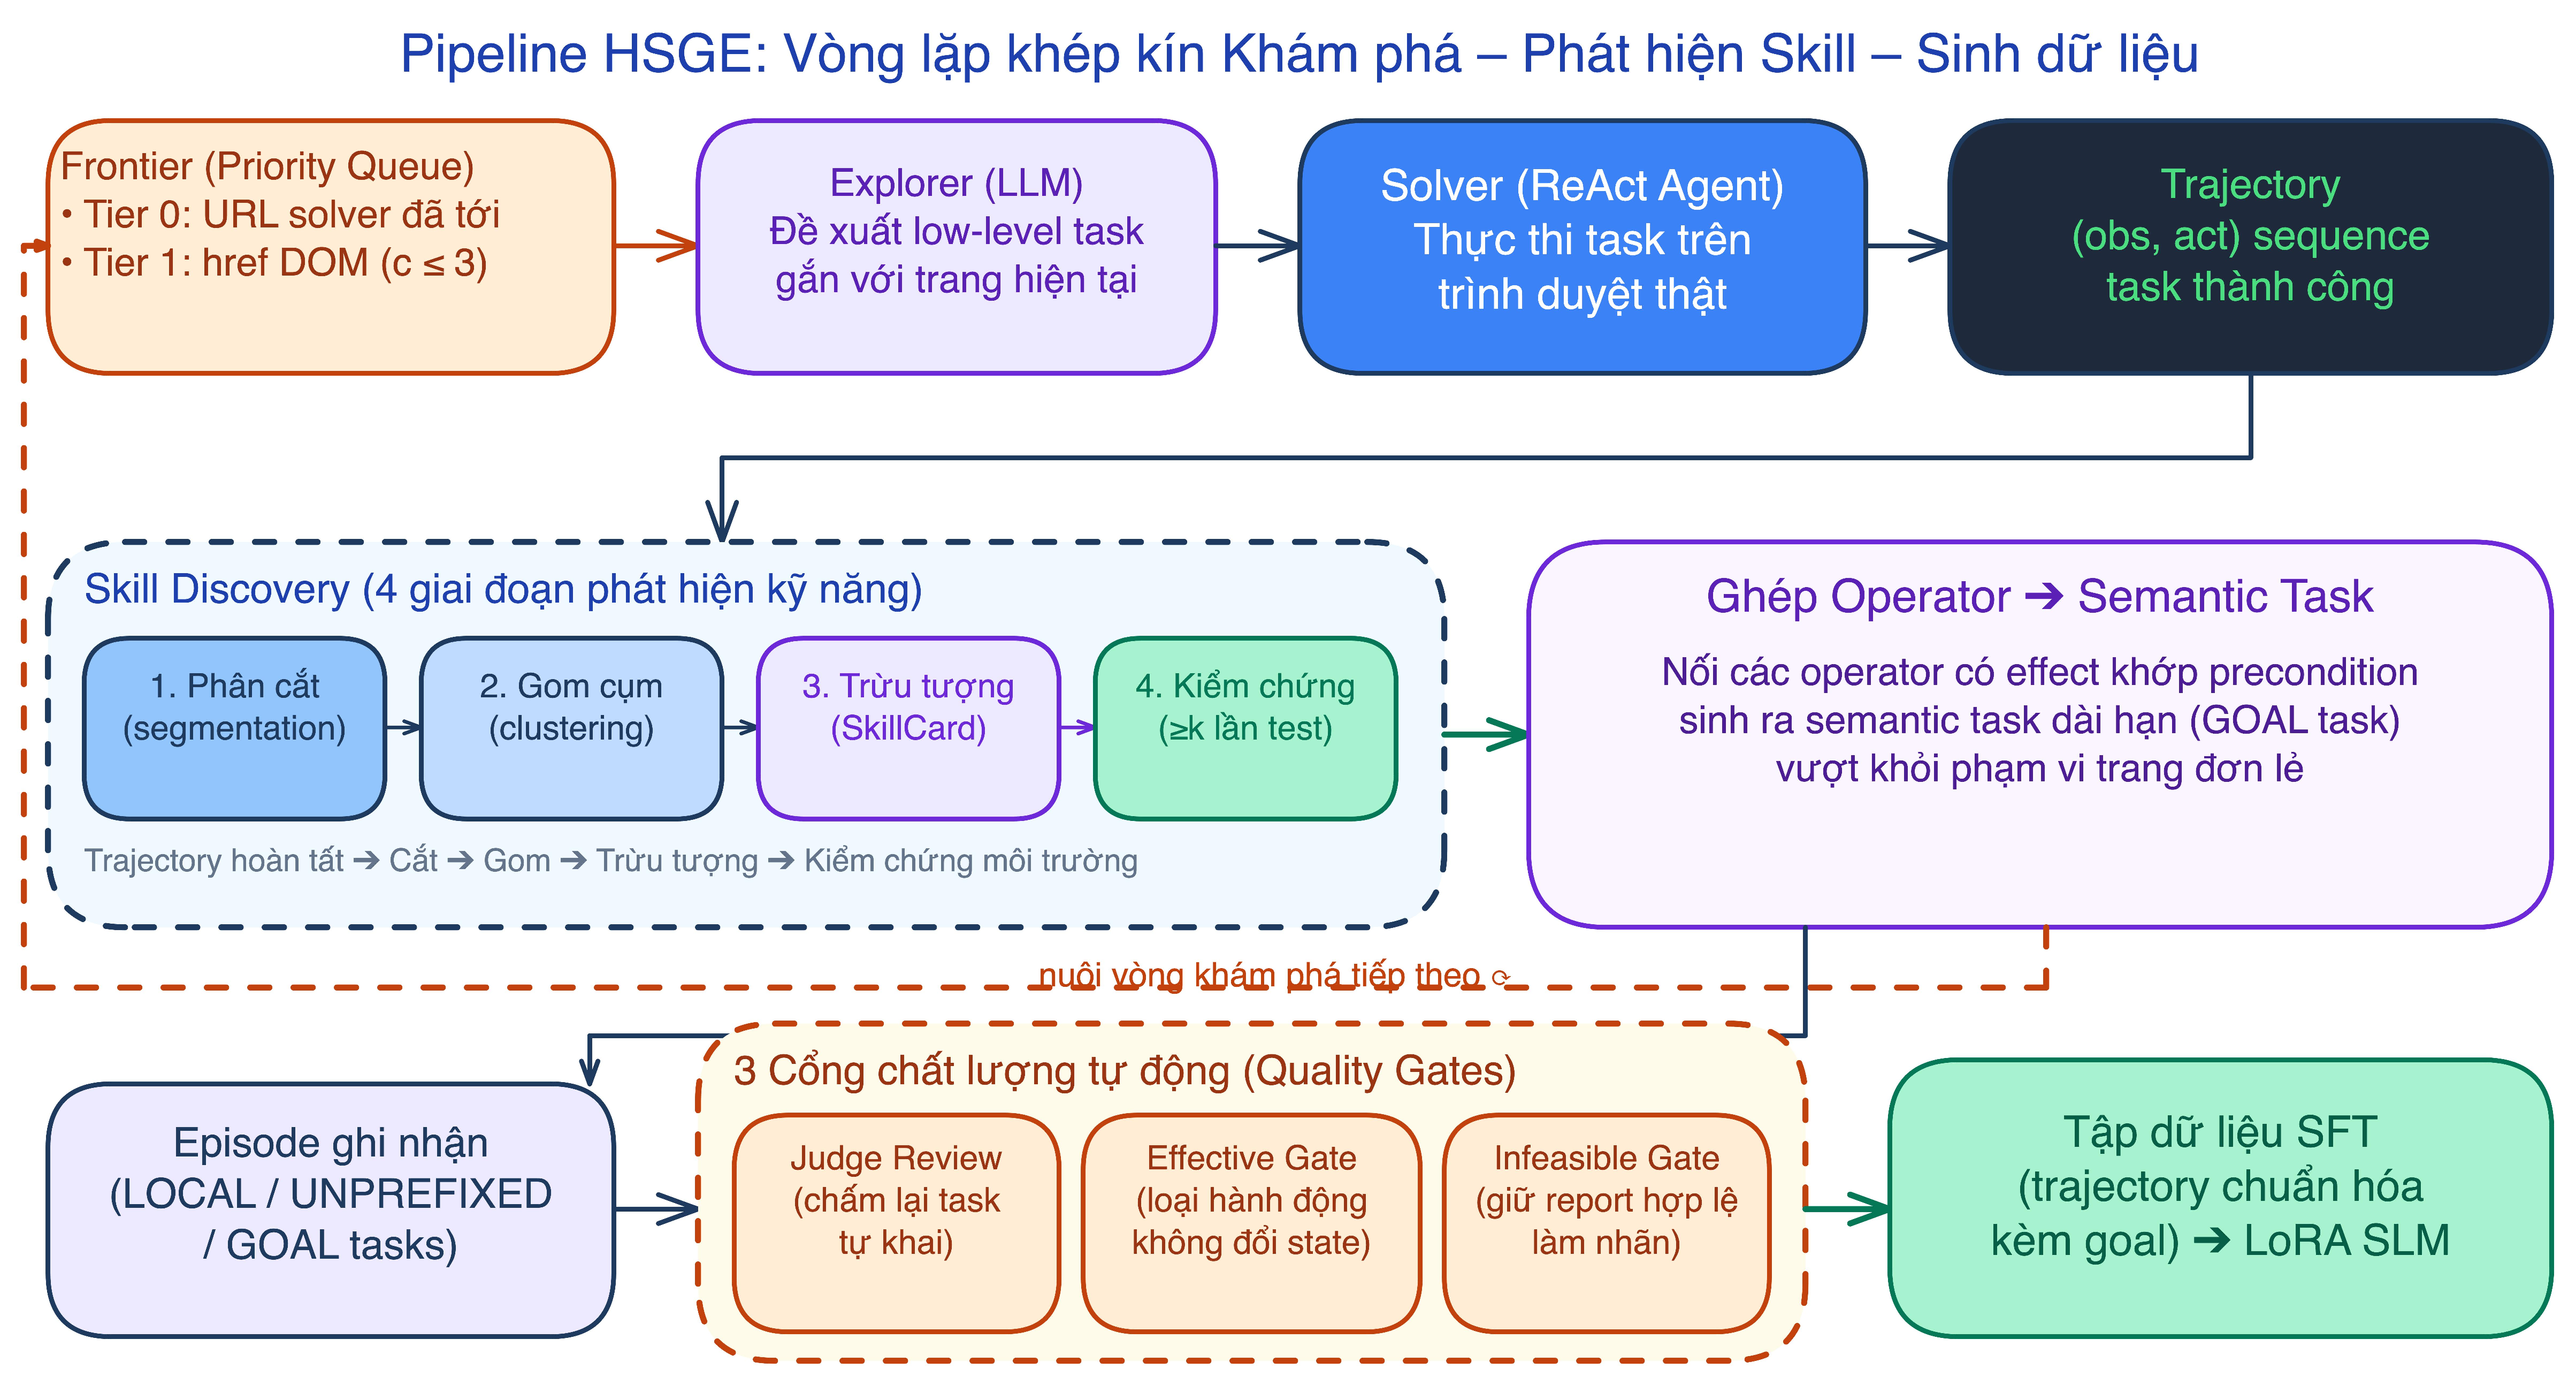
\includegraphics[width=\linewidth,height=0.86\textheight,keepaspectratio]{fig_pipeline.pdf}
  \end{center}
  \vspace{-0.1cm}
  \begin{center}
    \footnotesize
    \kw{Frontier} $\xrightarrow{\text{duyệt}}$ \textbf{Explorer/Solver} $\xrightarrow{\text{quy nạp}}$ \kw{Skill/Operator} $\xrightarrow{\text{ghép chuỗi}}$ \textbf{Semantic Task} $\xrightarrow{\text{lọc online}}$ \kw{Dataset SFT}
  \end{center}
\end{frame}

\subsection{Khám phá tự hành}
\begin{frame}{Khám phá tự hành: một vòng lặp trên một trang}
  \begin{columns}[onlytextwidth,t]
    \begin{column}{0.585\textwidth}
      \uncover<1->{
        \begin{hblock}{Năm bước của một vòng lặp}{\bhH}
          \begin{enumerate}\ilist
            \item \textbf{Lấy trang}: pop URL khỏi \kw{Frontier}, mở browser, đọc \kw{AXTree}.
            \item \textbf{Sinh task}: Explorer đề xuất $\le 9$ task \kw{từ chính trang đó} (INFO / NAV / MOD).
            \item \textbf{Giải task}: Solver chạy \kw{ReAct}, $15$ bước ($25$ nếu đa bước).
            \item \textbf{Kiểm định}: Judge soi trang đích; task đạt \kw{giải lại từ trang gốc}.
            \item \textbf{Mở rộng Frontier}: URL đã ghé $+$ liên kết trên trang.
          \end{enumerate}
        \end{hblock}
      }
    \end{column}

    \hfill
    \begin{column}{0.385\textwidth}
      \uncover<2->{
        \begin{hblock}{Bốn chốt chặn thoái hóa}{\bhH}
          \begin{itemize}\ilist
            \item \textbf{Node trùng}: băm nội dung AXTree $\rightarrow$ loại \kw{71/455} node.
            \item \textbf{Lặp thao tác}: dừng cứng khi cùng đích mà trang không đổi.
            \item \textbf{Bão hòa}: $\le 3$ node mỗi \kw{khuôn dạng} URL.
            \item \textbf{Task trùng}: nhớ task đã đề xuất, bỏ các bản gần trùng.
          \end{itemize}
        \end{hblock}
      }
    \end{column}
  \end{columns}

  \gap
  \uncover<3->{
    \begin{beamercolorbox}[wd=\textwidth,sep=2.5pt,leftskip=6pt,rightskip=6pt,rounded=true]{block body}
      \footnotesize \kw{Kết quả trên 4 website}: \kw{455} trang được khám phá, \kw{3.981} lượt thử, \kw{2.117} trajectory hợp lệ (\kw{53,2\%}).
    \end{beamercolorbox}
  }
\end{frame}

\subsection{Phát hiện Skill \& Quy nạp Operator}
\begin{frame}{Phát hiện skill và quy nạp operator}
  \begin{columns}[c]
    \begin{column}{0.48\textwidth}
      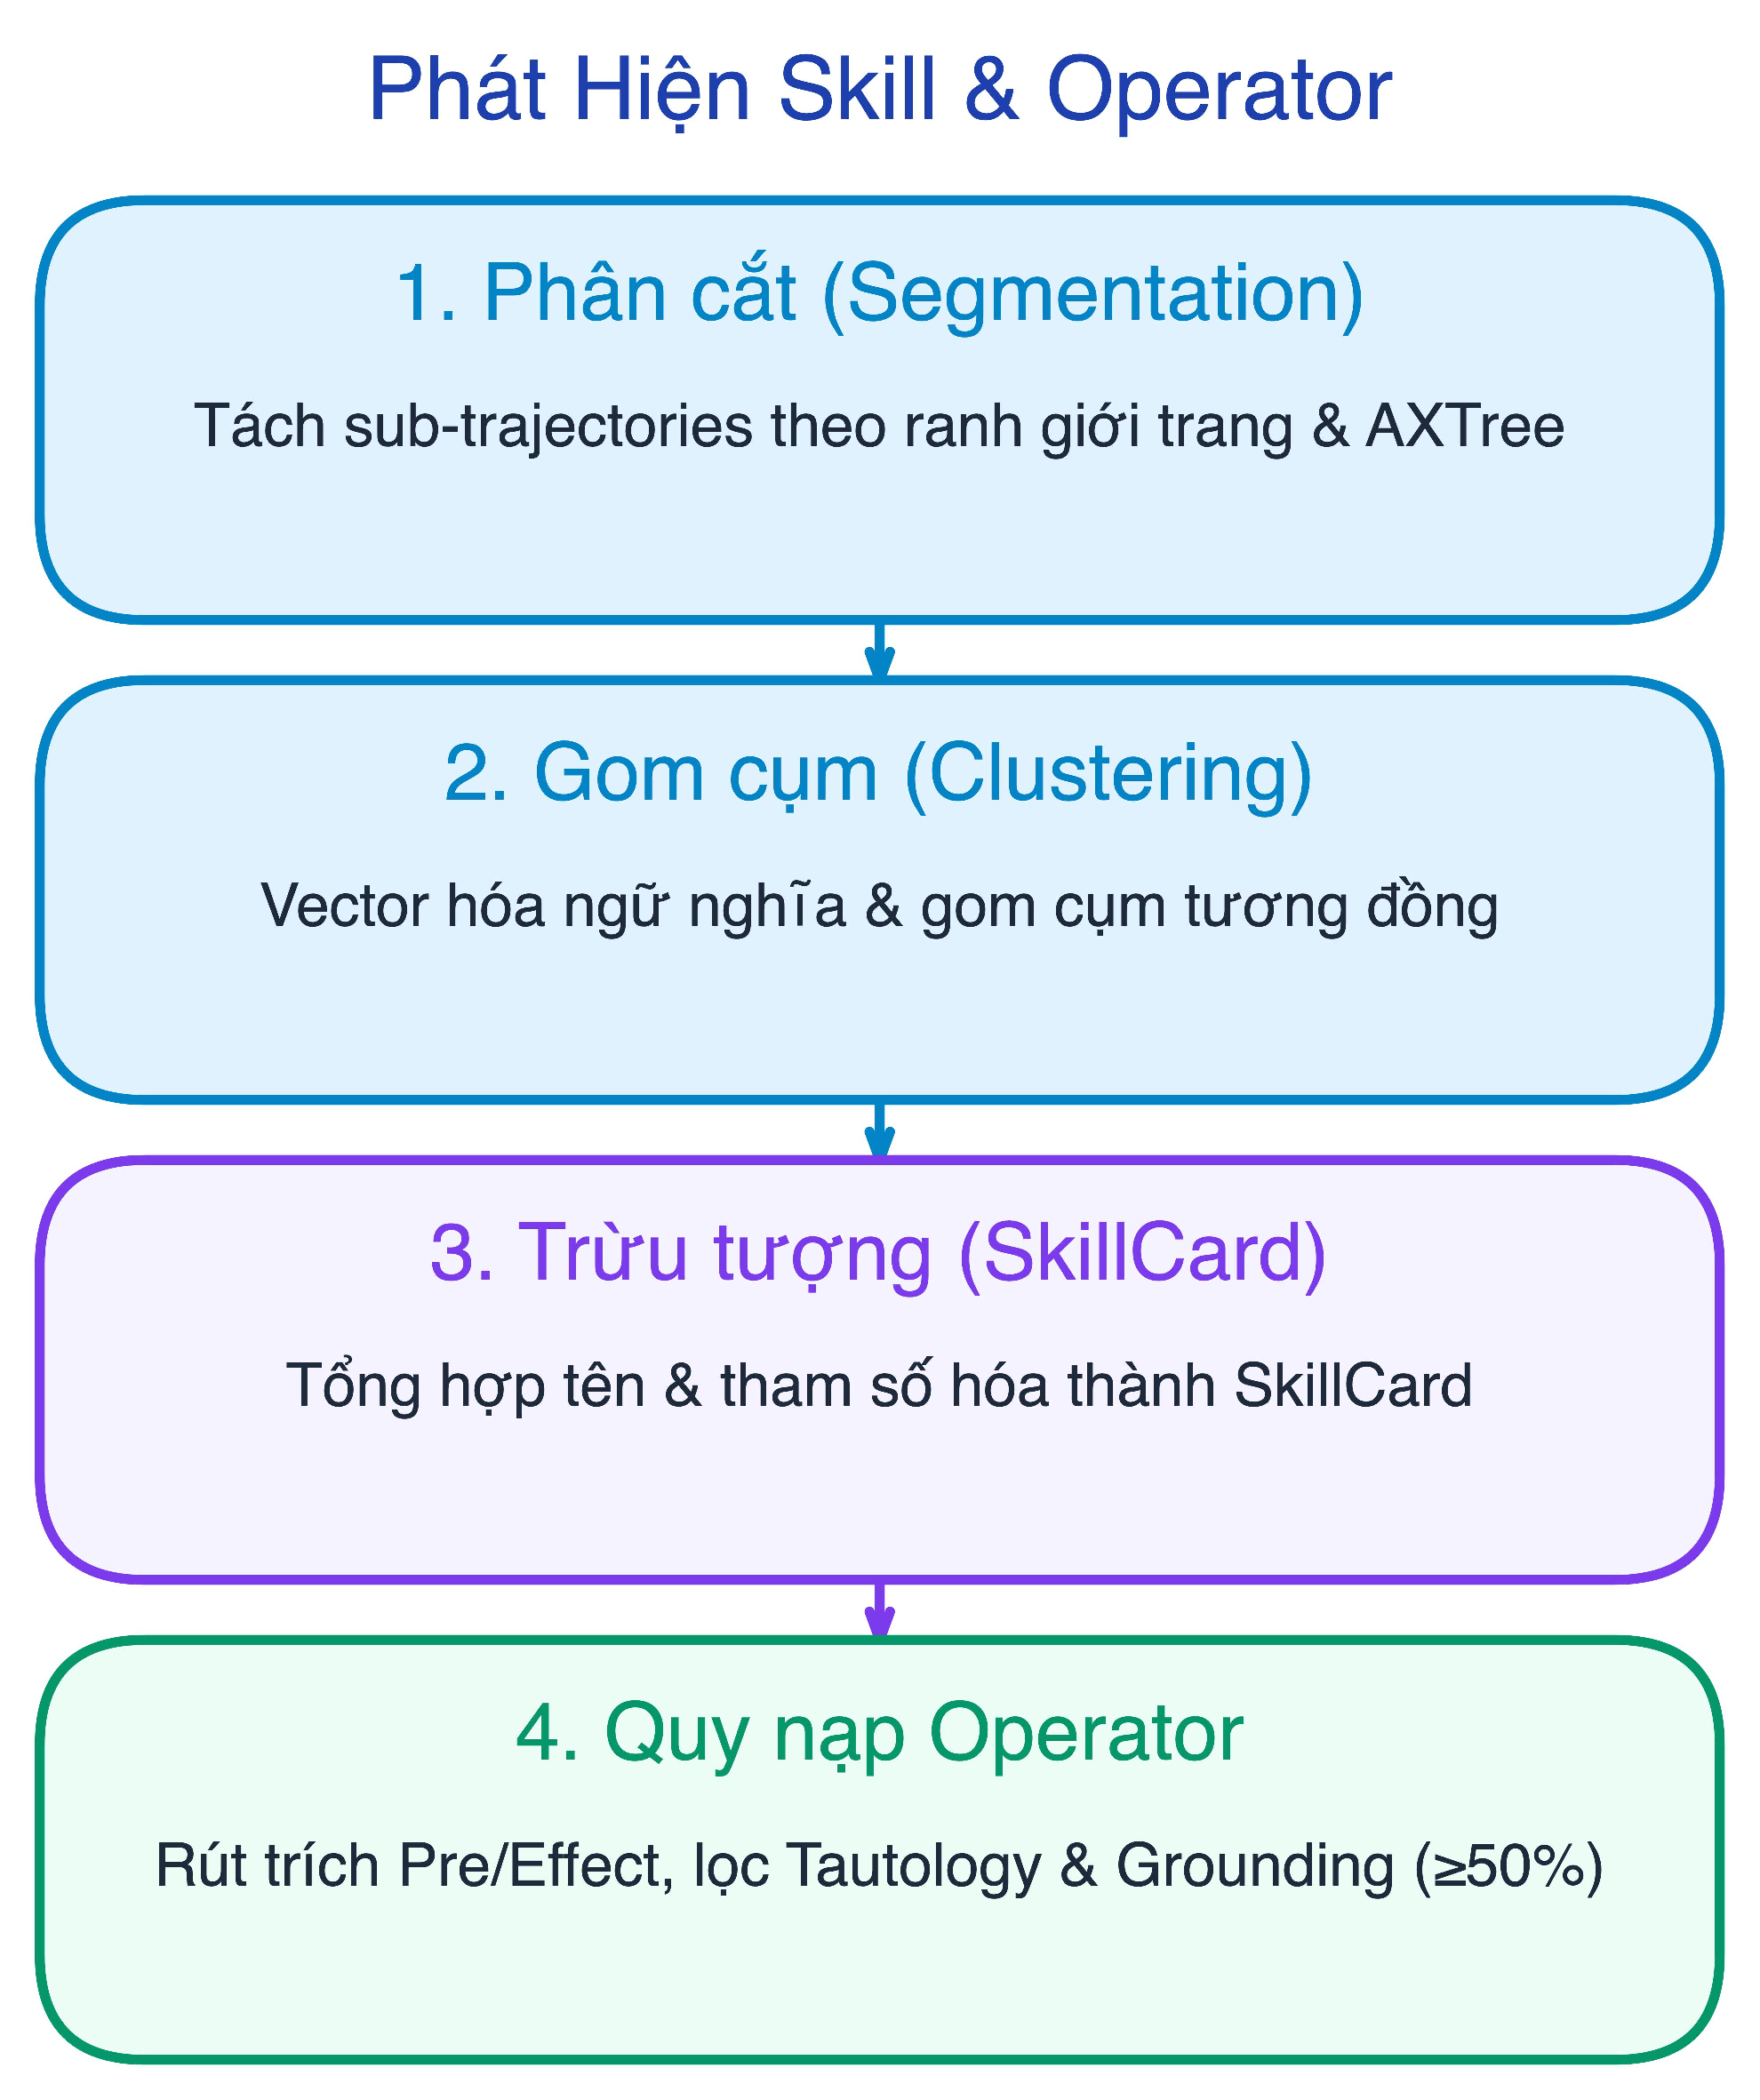
\includegraphics[width=\linewidth,height=0.85\textheight,keepaspectratio]{fig_discovery.pdf}
    \end{column}
    \hfill
    \begin{column}{0.50\textwidth}
      \uncover<1->{
        \head{4 bước phát hiện skill}
        \begin{enumerate}\ilist
          \item \textbf{Phân cắt}: đổi URL \& tụt tương đồng AXTree.
          \item \textbf{Gom cụm}: phi tham số (ngưỡng cosine).
          \item \textbf{Trừu tượng hóa}: \textit{SkillCard} tham số hóa.
          \item \textbf{Kiểm chứng}: chạy lại trong ngữ cảnh mới.
        \end{enumerate}
      }

      \vspace{0.1cm}
      \uncover<2->{
        \begin{block}{Quy nạp Operator \& Cổng chặn}
          \begin{itemize}\ilist
            \item \textbf{Chống trùng}: loại effect lặp lại precondition.
            \item \textbf{Grounding}: gỡ effect sai trên $\ge 50\%$ thành viên.
            \item $\Rightarrow$ \kw{146 skill} $\rightarrow$ \kw{57 operator}.
          \end{itemize}
        \end{block}
      }
    \end{column}
  \end{columns}
\end{frame}

\subsection{Sinh Semantic Task từ chuỗi Operator}
\begin{frame}{Sinh semantic task: ghép chuỗi operator}
  \begin{center}
    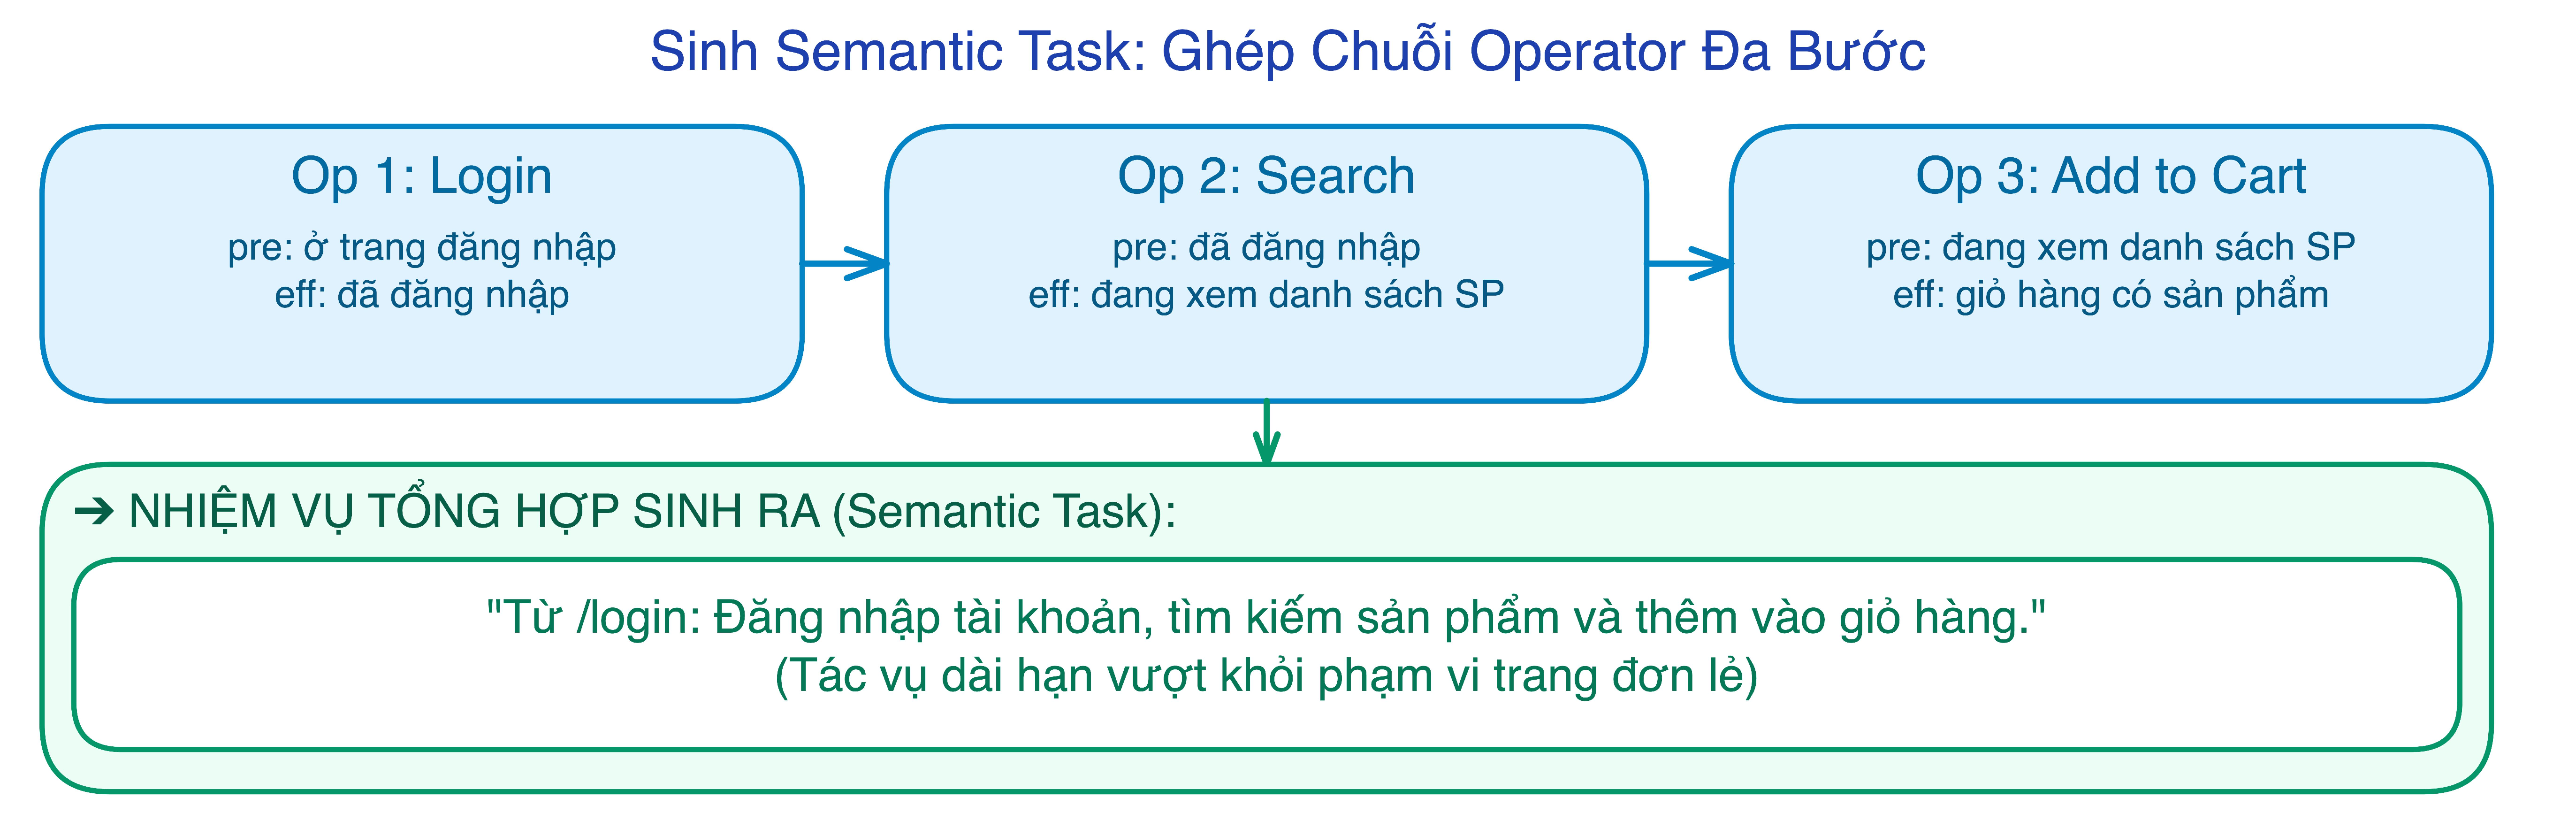
\includegraphics[width=0.95\linewidth,height=0.46\textheight,keepaspectratio]{fig_semantic.pdf}
  \end{center}
  \vspace{-0.15cm}
  \begin{columns}[t]
    \begin{column}{0.48\textwidth}
      \uncover<1->{
        \head{Hai cơ chế sinh tác vụ nhiều bước}
        \begin{itemize}\ilist
          \item \textbf{Bottom-up}: DFS đồ thị operator; chuỗi $\ge 2$ $\rightarrow$ task dài.
          \item \textbf{Top-down}: seed từ chức năng tổng quan website.
        \end{itemize}
      }
    \end{column}
    \hfill
    \begin{column}{0.48\textwidth}
      \uncover<2->{
        \begin{alertblock}{Kết quả thực thi}
          \footnotesize Sinh \kw{142 task} (130 seed + 12 chuỗi) $\rightarrow$ \kw{71 task thành công}.
        \end{alertblock}
      }
    \end{column}
  \end{columns}
\end{frame}

\subsection{Kiểm định trực tuyến \& Đóng gói SFT}
\begin{frame}{Kiểm định trực tuyến và đóng gói SFT}
  \begin{columns}[c]
    \begin{column}{0.46\textwidth}
      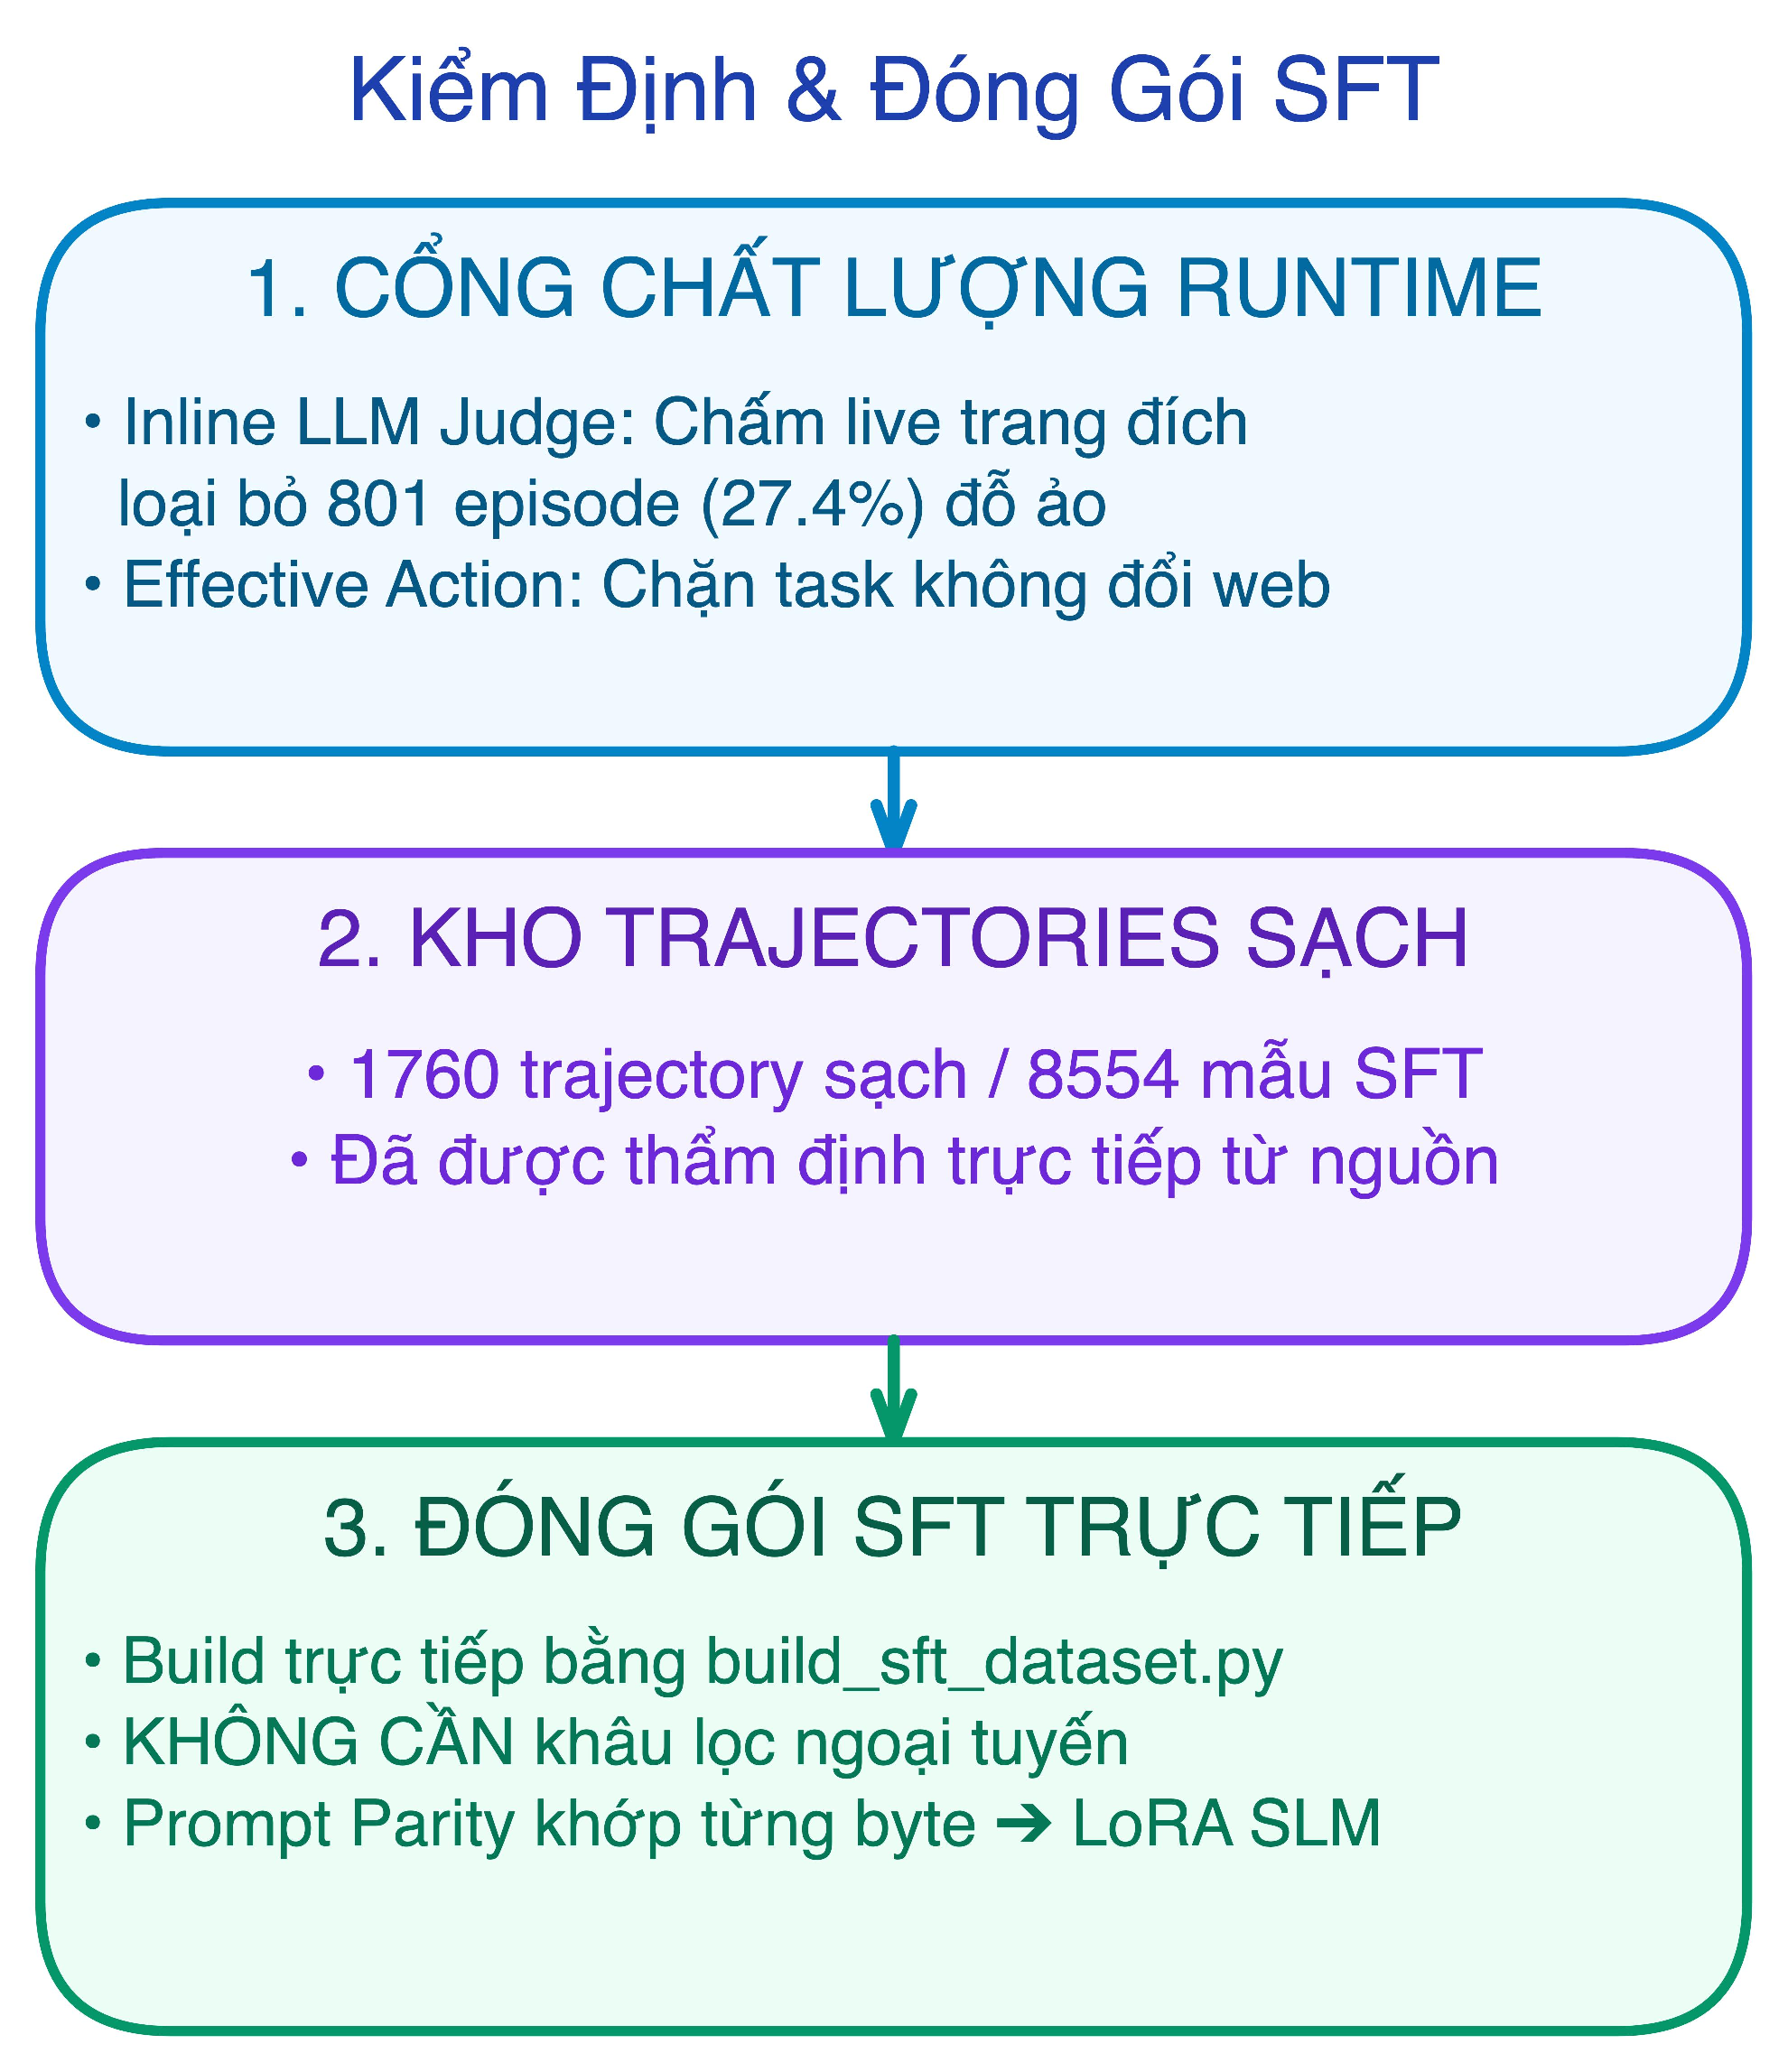
\includegraphics[width=\linewidth,height=0.85\textheight,keepaspectratio]{fig_curation.pdf}
    \end{column}
    \hfill
    \begin{column}{0.52\textwidth}
      \uncover<1->{
        \head{Kiểm soát chất lượng (Online Gates)}
        \begin{itemize}\ilist
          \item \textbf{Online LLM Judge}: chấm lại trang đích $\rightarrow$ loại \kw{801 episode (27,4\%)}.
          \item \textbf{Effective Action}: loại task không đổi trạng thái $\rightarrow$ \kw{1760 trajectory sạch}.
        \end{itemize}
      }

      \vspace{0.08cm}
      \uncover<2->{
        \begin{block}{Đóng gói SFT \& Prompt Parity}
          \begin{itemize}\ilist
            \item \textbf{Build trực tiếp}: sạch từ nguồn, không lọc ngoại tuyến.
            \item \textbf{Prompt Parity}: khớp từng byte train / suy luận.
            \item $\Rightarrow$ \kw{8554 train / 453 val} (0 trùng lặp).
          \end{itemize}
        \end{block}
      }
    \end{column}
  \end{columns}
\end{frame}


% !TEX root = ../main.tex

%%% ============================================================
\section{Thực nghiệm và kết quả}
%%% ============================================================

\subsection{Thiết lập \& Câu hỏi nghiên cứu}
\begin{frame}{Câu hỏi nghiên cứu và thiết lập thực nghiệm}
  \begin{columns}[t]
    \begin{column}{0.485\textwidth}
      \uncover<1->{
        \begin{block}{3 Câu hỏi nghiên cứu (RQ)}
          \begin{itemize}\scriptsize\setlength{\itemsep}{5pt}
            \item \textbf{CH1.} Khả năng tự động tạo tác vụ có ý nghĩa và quy mô tập dữ liệu thu được?
            \item \textbf{CH2.} Năng lực của SLM sau fine-tuning so với mô hình nền và các SOTA?
            \item \textbf{CH3.} Hiệu quả chi phí kinh tế của chu trình tự động sinh dữ liệu?
          \end{itemize}
        \end{block}
      }
    \end{column}
    \hfill
    \begin{column}{0.485\textwidth}
      \uncover<2->{
        \begin{block}{Thiết lập thực nghiệm}
          \begin{itemize}\scriptsize\setlength{\itemsep}{3.5pt}
            \item \textbf{Mô hình}: Base Qwen3.5-9B $\rightarrow$ HSGE-9B.
            \item \textbf{Fine-tuning}: LoRA / QLoRA (3 epoch, 1119 bước).
            \item \textbf{Đánh giá}: WebArena 655 task / 4 site, chấm bằng Task SR benchmark.
            \item \textbf{Đối chứng}: cùng prompt, cùng ngân sách bước với mô hình nền.
          \end{itemize}
        \end{block}
      }
    \end{column}

  \end{columns}
\end{frame}

\subsection{CH1: Tự động tạo tác vụ \& Quy mô dữ liệu}
\begin{frame}{CH1 - Tự động tạo tác vụ có ý nghĩa và quy mô dữ liệu}

  \begin{columns}[t,onlytextwidth]
    \begin{column}{0.53\textwidth}
      \vspace{-0.15cm}
      \setlength{\tabcolsep}{3pt}
      \begin{table}
        \scriptsize
        \begin{tabular}{@{}L{3.9cm} R{2.3cm}@{}}
          \toprule
          Quy mô khám phá & \textbf{4 site / 455 URL} \\
          Trajectory ghi nhận & \textbf{3.981 lượt thử} \\
          Trajectory hợp lệ & \textbf{2.117} (53,2\%) \\
          \midrule
          Tri thức tích lũy & \textbf{146 skills / 57 op} \\
          Semantic task & \textbf{142 task} \\
          \midrule
          Dữ liệu huấn luyện & \kw{1.760 trajectory} \\
          Dataset (Train / Val) & \kw{9.007 samples} (8.554 / 453) \\
          \bottomrule
        \end{tabular}
        \vspace{0.04cm}
        \centering
        \\ \scriptsize \textbf{Bảng 1: Quy mô dữ liệu sinh tự động HSGE}
      \end{table}
    \end{column}
    \hfill
    \begin{column}{0.45\textwidth}
      \vspace{-0.15cm}
      \begin{block}{Cổng kiểm soát chất lượng}
        \begin{itemize}\scriptsize\setlength{\itemsep}{0.5pt}
          \item \textbf{LLM-as-Judge}: Loại \kw{801 lượt (27,4\%)} dương tính giả.
          \item \textbf{Effective Action Gate}: Loại \kw{104 trajectory} DOM rỗng.
        \end{itemize}
      \end{block}

      \vspace{-0.25cm}
      \begin{block}{Kết quả thu hoạch}
        \begin{itemize}\scriptsize\setlength{\itemsep}{0.5pt}
          \item Sinh \kw{142 task} từ chuỗi operator.
          \item Thu hoạch \kw{1.760 trajectory sạch} (9.007 mẫu).
        \end{itemize}
      \end{block}
    \end{column}
  \end{columns}

  \vspace{-0.05cm}
  \begin{beamercolorbox}[wd=\textwidth,sep=2.5pt,leftskip=6pt,rightskip=6pt,rounded=true]{block body}
    \scriptsize \kw{Kết luận CH1}: HSGE tự động sinh tác vụ có ý nghĩa và thu hoạch 9.007 mẫu SFT sạch hoàn toàn không cần gán nhãn thủ công.
  \end{beamercolorbox}
\end{frame}

\subsection{CH2: Năng lực của SLM sau fine-tuning}
\begin{frame}{CH2 - So sánh hiệu năng với các hệ thống SOTA}
  \centering
  \vspace{-0.1cm}
  \setlength{\tabcolsep}{4pt}
  \begin{table}
    \scriptsize
    \begin{tabular}{@{}L{4.8cm} R{1.7cm} R{1.2cm} R{1.2cm} R{1.2cm} R{1.2cm}@{}}
      \toprule
      \textbf{Mô hình} & \multicolumn{5}{c}{\textbf{Tỷ lệ thành công Task SR (\%)}} \\
      \cmidrule(lr){2-6}

      & \textbf{Tổng (4 site)} & \textbf{Shopping} & \textbf{Admin} & \textbf{Reddit} & \textbf{GitLab} \\
      \midrule
      \multicolumn{6}{@{}l}{\textit{Mô hình đóng}} \\
      GPT-4o-mini [Gandhi et al.] & 20{,}0 & 19{,}3 & 19{,}2 & 21{,}1 & 20{,}9 \\
      GPT-4o [Gandhi et al.] & 37{,}5 & 32{,}3 & 35{,}7 & 50{,}9 & 36{,}7 \\
      \midrule
      \multicolumn{6}{@{}l}{\textit{Mô hình mở, cỡ nhỏ ($<10$B)}} \\
      Qwen-2.5-7B-Instruct  & 8{,}3 & 9{,}4 & 7{,}1 & 7{,}9 & 8{,}7 \\
      NNetNav-7B [Murty et al.] & 19{,}1 & 20{,}3 & 14{,}3 & 23{,}7 & \textbf{19{,}9} \\
      Go-Browse-7B [Gandhi et al.] & 22{,}6 & 22{,}4 & \textbf{25{,}3} & 30{,}7 & 15{,}3 \\
      \midrule
      Qwen3.5-9B (Mô hình nền) & 13{,}3 & 19{,}8 & 12{,}6 & 6{,}6 & 11{,}1 \\
      HSGE-7B (Qwen-2.5-7B FT) & 16{,}5 & 21{,}4 & 11{,}5 & 23{,}6 & 12{,}2 \\
      \textbf{HSGE-9B (Khóa luận)} & \textbf{24{,}6} & \textbf{28{,}3} & 21{,}4 & \textbf{34{,}0} & 18{,}3 \\
      \bottomrule
    \end{tabular}
    \vspace{0.08cm}
    \centering
    \\ \scriptsize \textbf{Bảng 2: So sánh tỷ lệ thành công Task SR (\%) với các hệ thống SOTA trên WebArena}
  \end{table}
\end{frame}

\begin{frame}{CH2 - So sánh mô hình nền (Base) và fine-tuning theo Website}
  \centering
  \vspace{-0.25cm}
  \setlength{\tabcolsep}{3pt}
  \begin{table}
    \scriptsize
    \begin{tabular}{@{}L{2.3cm} R{2.4cm} R{2.7cm} R{1.9cm} R{2.1cm}@{}}
      \toprule
      \textbf{Website} & \textbf{Base (SR, \%)} & \textbf{Fine-tuned (SR, \%)} &
      \textbf{$\Delta$ SR (đpt)} & \textbf{$p$ (McNemar)} \\
      \midrule
      Shopping       & 37/187 $=$ 19,8 & 53/187 $=$ 28,3 & $+$8,6  & 0,011 \\
      Reddit         & 7/106 $=$ 6,6   & 36/106 $=$ 34,0 & $+$27,4 & $<$0,001 \\
      GitLab         & 20/180 $=$ 11,1 & 33/180 $=$ 18,3 & $+$7,2  & 0,011 \\
      Shopping Admin & 23/182 $=$ 12,6 & 39/182 $=$ 21,4 & $+$8,8  & 0,005 \\
      \midrule
      \textbf{Tổng} & \textbf{87/655 $=$ 13,3} & \textbf{161/655 $=$ 24,6} &
      \kw{$+$11,3} & \kw{$<$0,001} \\
      \bottomrule
    \end{tabular}
    \vspace{0.02cm}
    \centering
    \\ \scriptsize \textbf{Bảng 3: Đối chứng mô hình nền Qwen3.5-9B và mô hình sau Fine-tune theo 4 Website}
  \end{table}

  \vspace{-0.45cm}
  \begin{columns}[t,onlytextwidth]
    \begin{column}{0.49\textwidth}
      \begin{alertblock}{Phân tích kết quả}
        \begin{itemize}\scriptsize\setlength{\itemsep}{0pt}
          \item \textbf{Cú pháp}: Lỗi định dạng giảm từ 26,0\% $\rightarrow$ \kw{0,6\%}.
          \item \textbf{Ra quyết định}: SR chuẩn cú pháp tăng \kw{17,9\% $\rightarrow$ 23,5\%} ($p=0{,}003$).
        \end{itemize}
      \end{alertblock}
    \end{column}
    \hfill
    \begin{column}{0.49\textwidth}
      \begin{block}{Ý nghĩa thống kê McNemar}
        \begin{itemize}\scriptsize\setlength{\itemsep}{0pt}
          \item \textbf{Vượt trội Base}: \kw{100 task độc quyền} HSGE giải được (Base chỉ 26 task).
          \item \textbf{Ý nghĩa thống kê}: Đạt \kw{$p < 0{,}001$} trên toàn bộ 4 website.
        \end{itemize}
      \end{block}
    \end{column}
  \end{columns}

  \vspace{-0.15cm}
  \begin{beamercolorbox}[wd=\textwidth,sep=2.5pt,leftskip=6pt,rightskip=6pt,rounded=true]{block body}
    \scriptsize \kw{Kết luận CH2}: Fine-tuning nâng Task SR lên 24,6\% ($+11,3\%$, $p < 0{,}001$), làm chủ cả cú pháp lẫn ra quyết định, đạt mức SOTA $<10$B.
  \end{beamercolorbox}
\end{frame}

\subsection{CH3: Hiệu quả chi phí trong tự động tạo dữ liệu}
\begin{frame}{CH3 - Hiệu quả chi phí trong quá trình tự động tạo dữ liệu}
  \vspace{-0.15cm}
  \begin{columns}[t,onlytextwidth]
    \begin{column}{0.49\textwidth}
      \begin{block}{Chi phí API toàn chu trình \& Token}
        \begin{itemize}\scriptsize\setlength{\itemsep}{2pt}
          \item \textbf{OpenAI API}: \$42,29 (\texttt{solver}, \texttt{explorer}).
          \item \textbf{DeepSeek API}: \$11,92 (\texttt{judge}, pipeline skill).
          \item \textbf{Tổng chi phí API}: \kw{\$54,21} ($<$ \$14 / site).
          \item \textbf{Đơn giá / trajectory}: \kw{\$0,0308} / trajectory.
          \item \textbf{Lời gọi API}: \kw{20.808 lượt} LLM (Solver \kw{85,5\%}).
          \item \textbf{Tối ưu token}: Chuyển sang GPT-5.6-luna giúp giảm đơn giá token đầu vào \kw{$\sim$12 lần} so với GPT-4o.
        \end{itemize}
      \end{block}
    \end{column}
    \hfill
    \begin{column}{0.48\textwidth}
      \begin{block}{So sánh hiệu quả chi phí với Go-Browse}
        \centering
        \vspace{-0.1cm}
        \setlength{\tabcolsep}{3pt}
        \scriptsize
        \begin{tabular}{@{}L{2.3cm} R{3.3cm}@{}}
          \toprule
          \textbf{Phương pháp} & \textbf{Chi phí API / Trajectory} \\
          \midrule
          Go-Browse-7B & \$0,1026 \\
          \textbf{HSGE (Khóa luận)} & \kw{\$0,0308} \\
          \midrule
          \textbf{Tỷ lệ tiết kiệm} & \kw{Rẻ hơn 3,3 lần} \\
          \bottomrule
        \end{tabular}

        \vspace{0.02cm}
        \scriptsize \textbf{Bảng 4: So sánh đơn giá API trajectory tự động tạo}
      \end{block}

      \vspace{-0.25cm}
      \begin{block}{Ý nghĩa kinh tế}
        \begin{itemize}\scriptsize\setlength{\itemsep}{1pt}
          \item Khẳng định tính khả thi với tài nguyên giới hạn.
          \item Chu trình HSGE nằm trong ngân sách nhóm nhỏ.
        \end{itemize}
      \end{block}
    \end{column}
  \end{columns}

  \vspace{0.05cm}
  \begin{beamercolorbox}[wd=\textwidth,sep=2.5pt,leftskip=6pt,rightskip=6pt,rounded=true]{block body}
    \scriptsize \kw{Kết luận CH3}: Chi phí API tự tạo dữ liệu \$0,0308/trajectory (rẻ hơn Go-Browse 3,3 lần), chứng minh tính khả thi kinh tế vượt trội cho nhóm nhỏ.
  \end{beamercolorbox}
\end{frame}


% Kết luận & Hỏi đáp: mục kết thúc phần trình bày chính (không có phụ lục)
\AtBeginSection[]{}
% !TEX root = ../main.tex

%%% ============================================================
\section{Kết luận \& Hỏi đáp}
%%% ============================================================

\subsection{Đóng góp chính \& Hướng phát triển}
\begin{frame}{Đóng góp chính và hướng phát triển}
  \begin{columns}[t,onlytextwidth]
    \begin{column}{0.49\textwidth}
      \uncover<1->{
        \begin{block}{Đóng góp chính của khóa luận}
          \begin{itemize}\scriptsize\setlength{\itemsep}{3pt}
            \item \textbf{Về Khoa học}: Đề xuất kiến trúc đồ thị 2 tầng (State Graph $\leftrightarrow$ Operator Graph), thuật toán phát hiện skill, quy nạp operator và ghép chuỗi sinh semantic task đa bước.
            \item \textbf{Về Thực tiễn}: Cung cấp pipeline tự động hóa hoàn chỉnh, bộ dataset \kw{9.007 mẫu SFT} và mô hình HSGE-9B đạt \kw{24,6\%} Task SR với chi phí chỉ \kw{\$0,0308/trajectory} (\kw{rẻ hơn 3,3 lần} so với Go-Browse).
            \item \textbf{Tài nguyên mở}: Mã nguồn pipeline, dữ liệu huấn luyện và trọng số mô hình HSGE-9B.
          \end{itemize}
        \end{block}
      }


    \end{column}
    \hfill
    \begin{column}{0.49\textwidth}
      \uncover<2->{
        \begin{block}{Hướng phát triển tương lai}
          \begin{itemize}\scriptsize\setlength{\itemsep}{3.5pt}
            \item \textbf{Khôi phục lỗi tự động}: Tự sửa lỗi và thử lại khi gặp sự cố giao diện (timeout, kẹt trang DOM).
            \item \textbf{Tối ưu khám phá với RL}: Kết hợp Học tăng cường (RL) giúp Explorer tự học chiến lược duyệt web tối ưu.
            \item \textbf{Học từ thất bại}: Khai thác trajectory thất bại thông qua DPO / Preference Learning.
            \item \textbf{Tổng quát hóa}: Mở rộng pipeline khám phá cho các ứng dụng ngoài miền (cross-domain).
          \end{itemize}
        \end{block}
      }
    \end{column}
  \end{columns}
\end{frame}


\begin{frame}[plain]
  \centering
  \vfill
  % `title` fg is white in the whale colortheme (it sits on the dark title bar), so on a
  % [plain] frame it rendered white-on-white; structure.fg is the theme's dark blue.
  {\usebeamerfont{title}\color{structure.fg}\Large\textbf{XIN CẢM ƠN HỘI ĐỒNG}}\\[0.25cm]
  {\usebeamerfont{title}\color{structure.fg}\large\textbf{HỎI \& ĐÁP}}\\[0.25cm]
  {\normalsize Nhóm nghiên cứu sẵn sàng lắng nghe câu hỏi và góp ý}
  \vfill
  \footnotesize
  \begin{tabular}{ll}
    \textbf{Sinh viên thực hiện:} & Trương Bảo Kiệt (22127223) - Hồ Tiến Phát (22127321) \\
    \textbf{GVHD:} & PGS.TS. Nguyễn Văn Vũ \\
    \textbf{Đơn vị:} & Bộ môn CNPM, Khoa CNTT - Trường ĐH KHTN, ĐHQG-HCM
  \end{tabular}
  \vfill
\end{frame}




\end{document}
